%\subsection{Histogramm f\"ur Evaluation Method (88)}
%\begin{figure}
\begin{center}
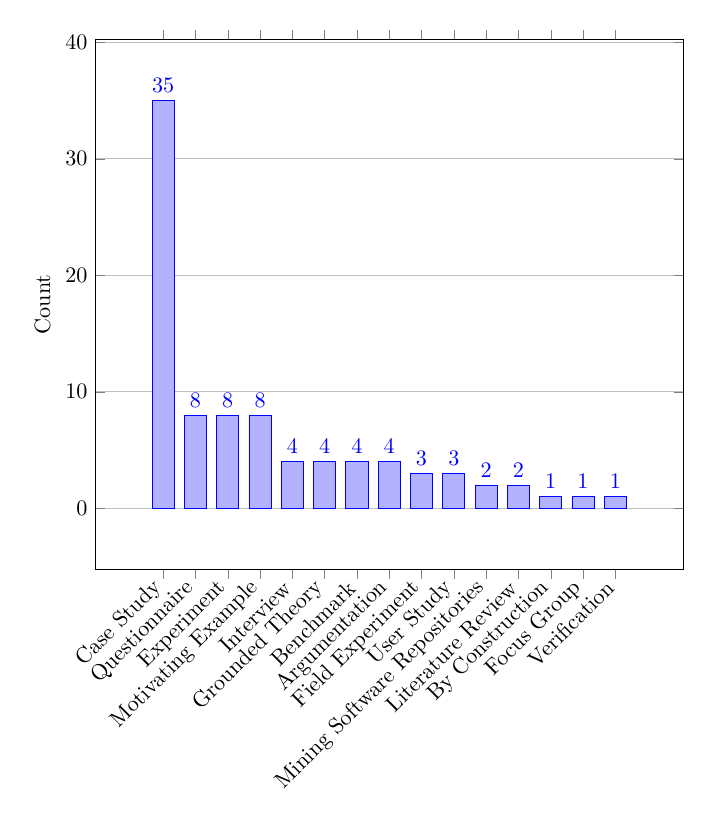
\begin{tikzpicture}[scale=.8]
\begin{axis}[ ybar, ymajorgrids, enlargelimits=0.15, legend style={at={(0.5,-0.15)}, anchor=north,legend columns=-1},
    width=.90\linewidth,height=10cm,
    nodes near coords, %nodes near coords align=below,
    ylabel={Count}, ymin=0,
    x tick label style={rotate=45,anchor=east},
    xtick={1,2,3,4,5,6,7,8,9,10,11,12,13,14,15},
    xticklabels={Case Study, Questionnaire, Experiment, Motivating Example, Interview, Grounded Theory, Benchmark, Argumentation, Field Experiment, User Study, Mining Software Repositories, Literature Review, By Construction,Focus Group,Verification
}
    %xlabel={Evaluation Method}    
    ]
  \addplot coordinates { (1,35)  (2,8)  (3,8)  (4,8)  (5,4)  (6,4)  (7,4)  (8,4)  (9,3)  (10,3)  (11,2)  (12,2)  (13,1)  (14,1)  (15,1)   };
\end{axis}
\end{tikzpicture}
\end{center}
%\caption{Histogramm f\"ur Evaluation Method (88)}
%\label{fig:histo_evaluationmethod}
%\end{figure}

